\documentclass{beamer}
\mode<presentation>
\usetheme[compress]{Berlin}
\usecolortheme{beaver}
\setbeamertemplate{navigation symbols}{}
\setbeamertemplate{footline}{}
\setbeamerfont{footnote}{size=\tiny}
\usepackage{hyperref}
\hypersetup{linkcolor=}

\title{Active Learning with Astronomical Data}
\subtitle{}
\institute{Supervisors: \\Cheng Soon Ong, Christian Wolf, Justin Domke}
\author[Alasdair Tran]{Alasdair Tran \\ \texttt{u4921817}}
\date{\footnotesize{19 June 2015}}
\setbeamertemplate{headline}{} % hide header

\begin{document}
	
\begin{frame}
	\titlepage
\end{frame}

% % % % % % % % % % % % % % % % % % % % % % % % % % % % % % % % % % % % % % % % % % % % % 
\section{Dataset}
\begin{frame}{Sloan Digital Sky Survey}
	Photometric measurements of 800 million objects, out of which
	3 million objects are spectroscopically labelled.
	\begin{figure}
		\centering
		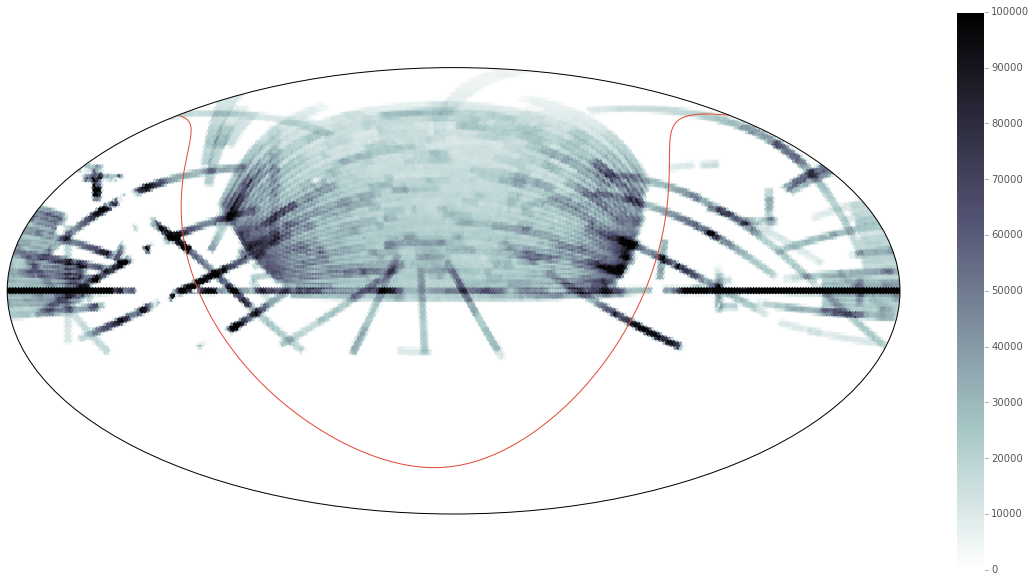
\includegraphics[width=\textwidth]{images/sdss_coverage}
		\caption{The coverage of the Sloan survey.}
	\end{figure}
\end{frame}


\begin{frame}{Photometry vs Spectroscopy}
	\begin{figure}
		\centering
		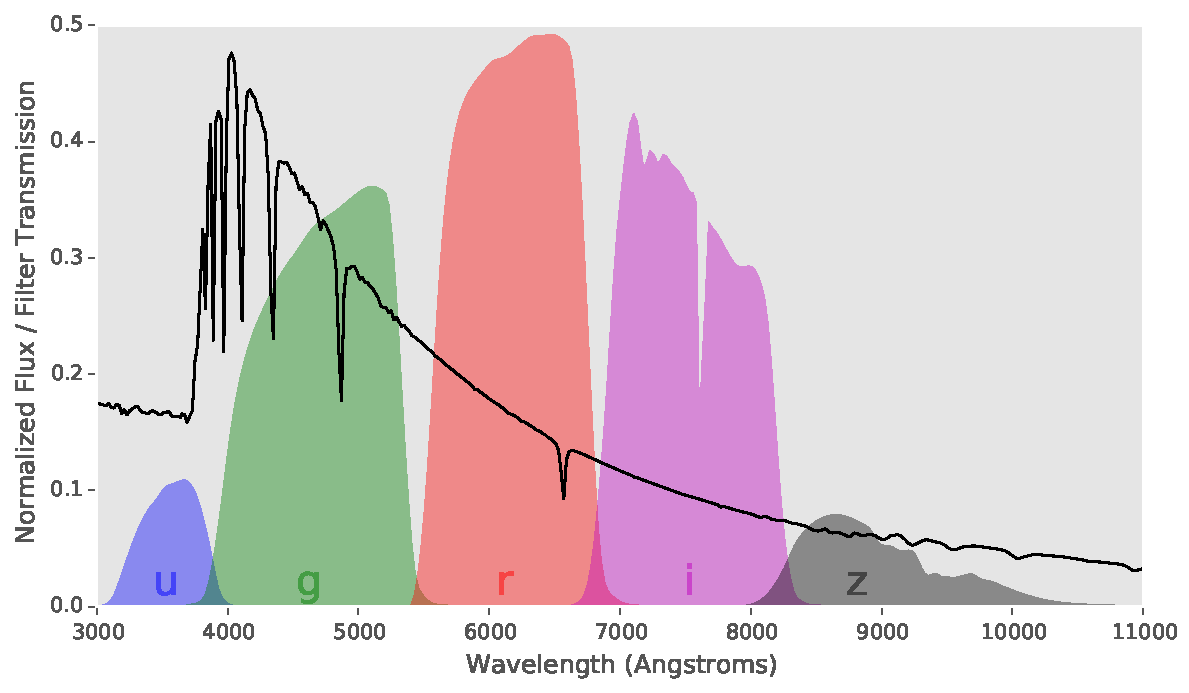
\includegraphics[width=\textwidth]{images/vega}
		\caption{SDSS Filters and Vega Spectrum}
	\end{figure}
\end{frame}


\begin{frame}{Improving the Features}
	\begin{figure}
		\centering
		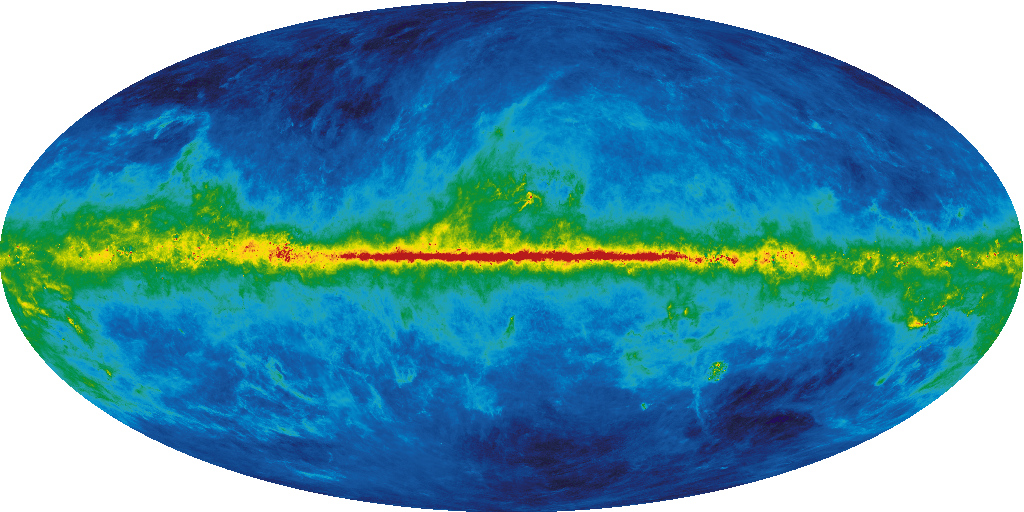
\includegraphics[width=\textwidth]{images/lrg_ebv_image}
		\caption{Map of Galactic Reddening, E(B-V), SFD (1998)\footnotemark}
	\end{figure}
\footnotetext[1]{Image from LAMBDA.}
\end{frame}

\begin{frame}{Improving the Features}
	\begin{columns}[T]
		\begin{column}{.45\textwidth}
			Magnitudes measurements:
			\begin{itemize}
				\item $u$-band
				\item $g$-band
				\item $r$-band
				\item $i$-band
				\item $z$-band
			\end{itemize}
		\end{column}
		\begin{column}{.45\textwidth}
			Colour measurements:
			\begin{itemize}
				\item $u-g$ index
				\item $g-r$ index
				\item $r-i$ index
				\item $i-z$ index
			\end{itemize}
		\end{column}
	\end{columns}
	\vspace{2em}
	Colour indices are independent of distance.
\end{frame}






% % % % % % % % % % % % % % % % % % % % % % % % % % % % % % % % % % % % % % % % % % % % %
\section{Classification}
\begin{frame}{Training Data}
	\begin{figure}
		\centering
		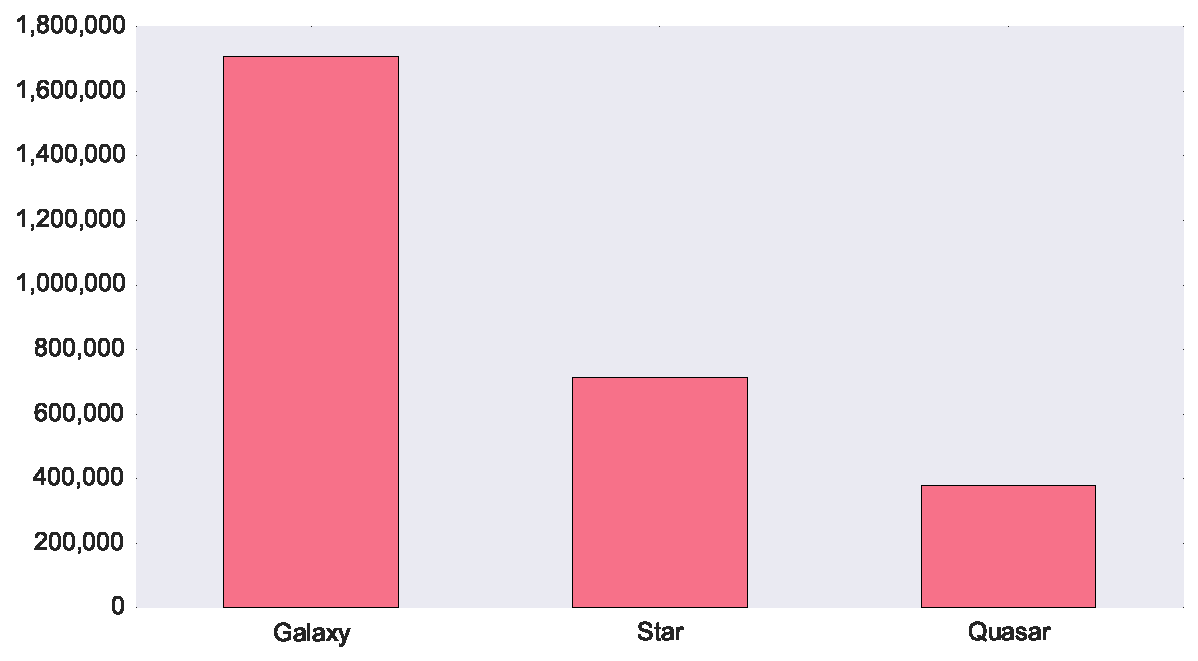
\includegraphics[width=\textwidth]{images/training_dist}
		\caption{Distribution of Classes in the Training Set.}
	\end{figure}
\end{frame}

\begin{frame}{Learning Curves}
	\begin{figure}
		\centering
		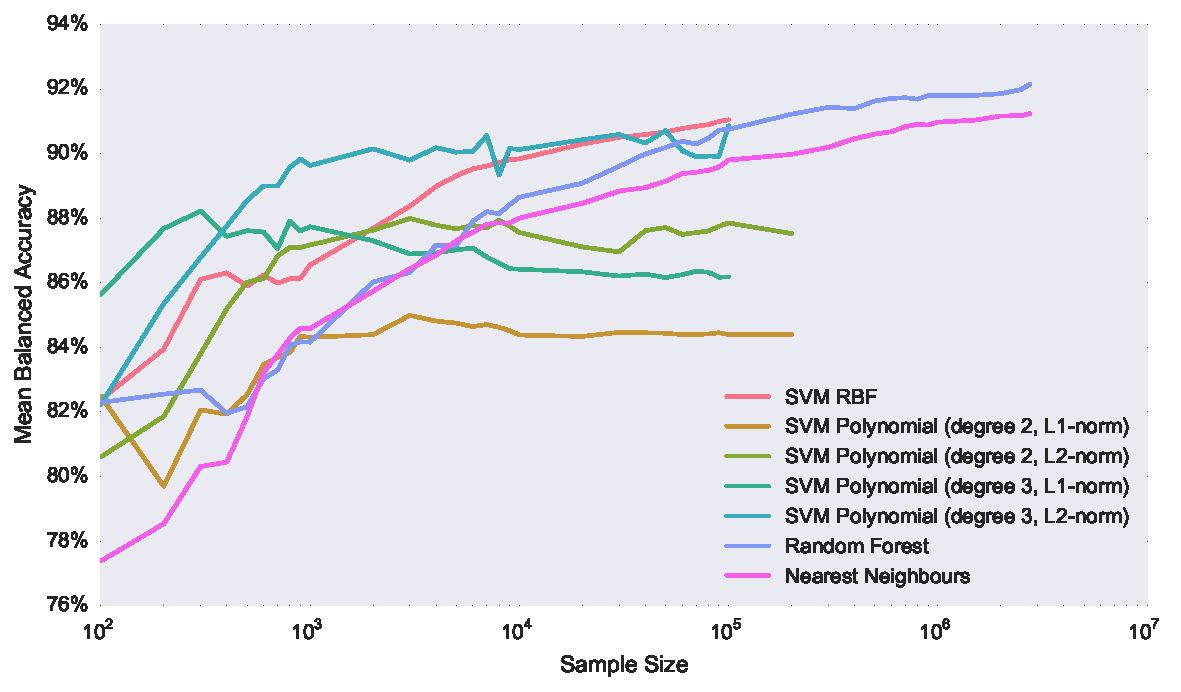
\includegraphics[width=\textwidth]{images/learning_curves}
		\caption{Learning Curves of Various Classifiers.}
	\end{figure}
\end{frame}


\begin{frame}{Predicting with Test Data}
99\% of galaxies are correctly classified.
	\begin{figure}
		\centering
		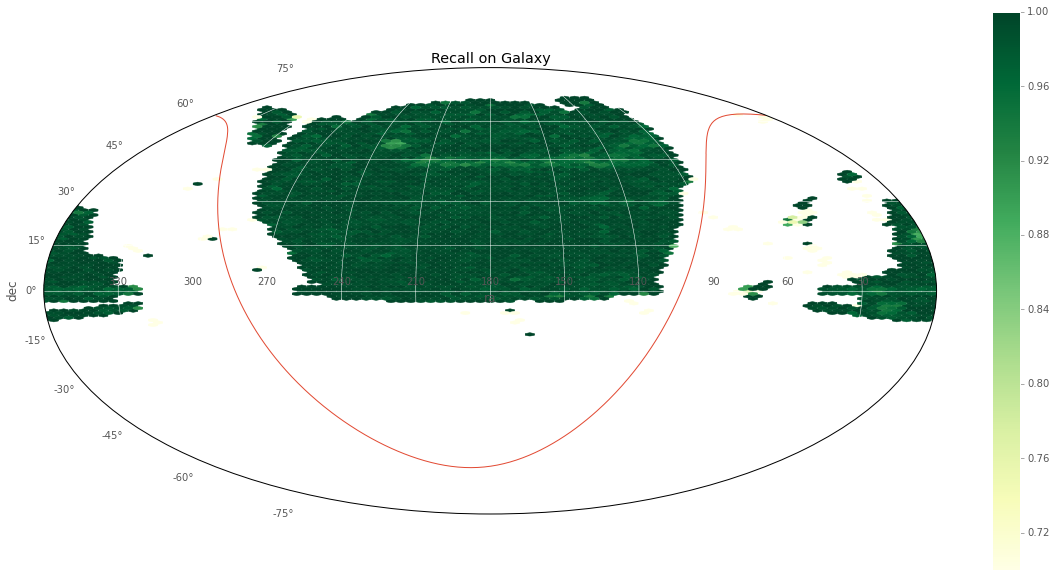
\includegraphics[width=\textwidth]{images/recall_galaxies}
		\caption{Random Forest's Recall on Galaxies.}
	\end{figure}
\end{frame}


\begin{frame}{Predicting with Test Data}
	6\% of stars are misclassified as quasars.
	\begin{figure}
		\centering
		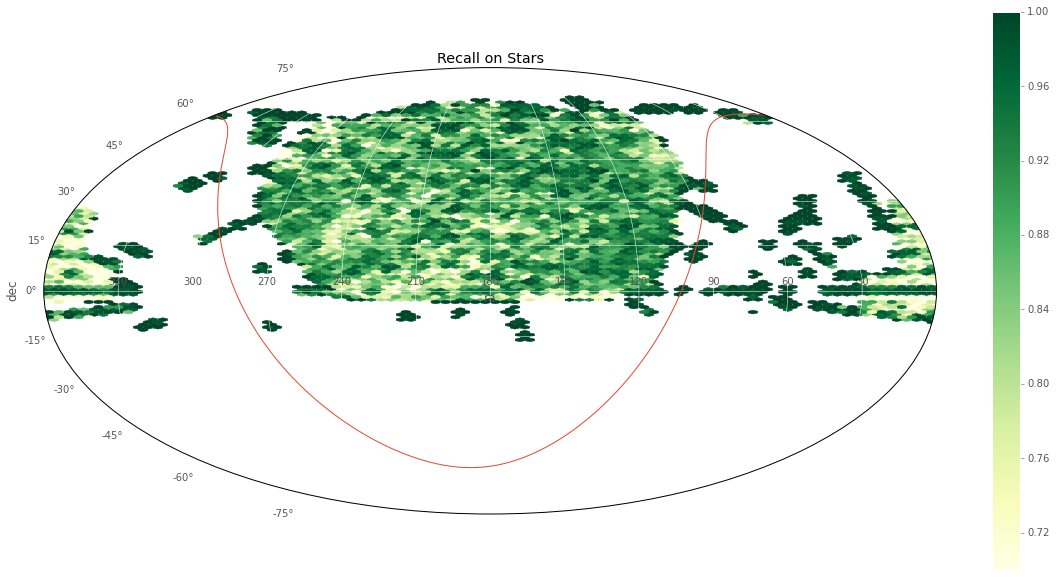
\includegraphics[width=\textwidth]{images/recall_stars}
		\caption{Random Forest's Recall on Stars.}
	\end{figure}
\end{frame}

\begin{frame}{Predicting with Test Data}
	8\% of quasars are misclassified as stars.
	\begin{figure}
		\centering
		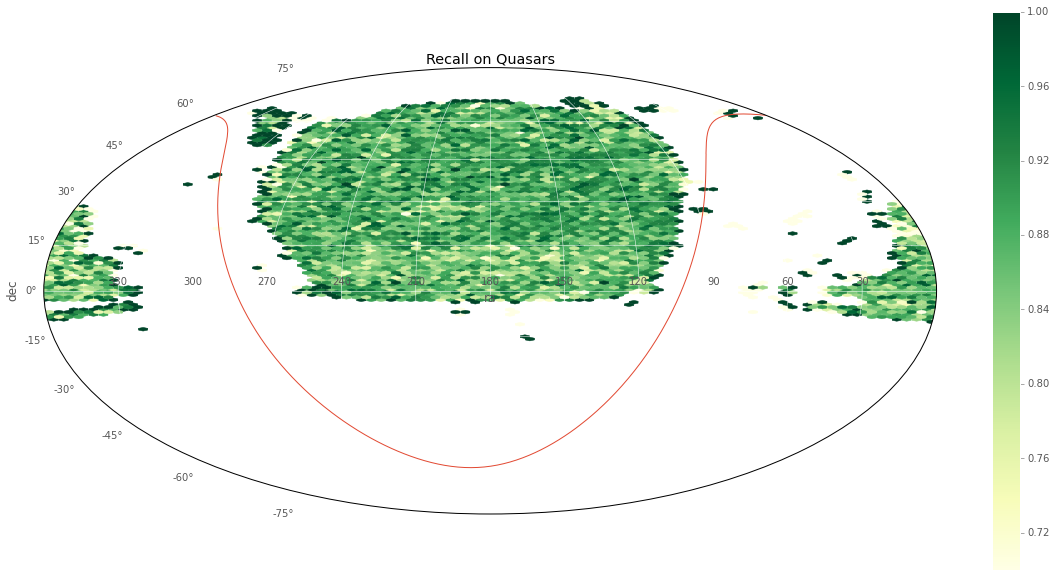
\includegraphics[width=\textwidth]{images/recall_quasars}
		\caption{Random Forest's Recall on Quasars.}
	\end{figure}
\end{frame}


\begin{frame}{Predicting Unknowns}
	\begin{figure}
		\centering
		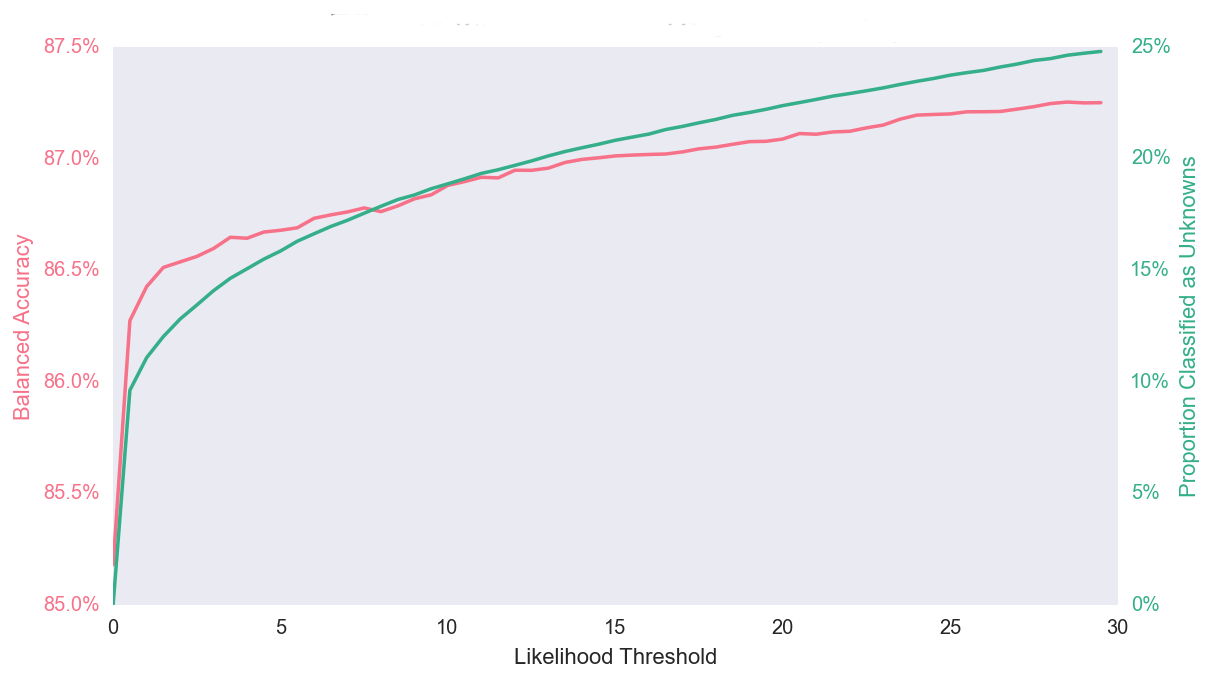
\includegraphics[width=\textwidth]{images/unknowns}
		\caption{Effect of the Likelihood Threshold (QDA).}
	\end{figure}
\end{frame}




% % % % % % % % % % % % % % % % % % % % % % % % % % % % % % % % % % % % % % % % % % % % %
\section{Active Learning}
\begin{frame}{Active Learning: Motivation}
	\begin{itemize}
		\item Labelling is expensive.
		\item One solution is to actively query the expert to obtain the training set.
		\item The goal is to beat random sampling.
	\end{itemize}
\end{frame}

\begin{frame}{Active Learning: Algorithm}
	Start with a partial training set and an unlabelled pool.\\
	Repeat the following until we have enough training data:
	\begin{enumerate}
		\item Select $T$ random examples from the pool.
		\item Rank these $T$ examples according to an \textbf{active learning rule}.
		\item Give the expert the highest-ranked example for labelling.
		\item Add this new labelled example to the training set.
		\item Retrain \textbf{the classifier}.
	\end{enumerate}
\end{frame}

\begin{frame}{Active Learning: Uncertainty Sampling Heuristics}
	\begin{itemize}
		\item Pick the example whose prediction vector $p$ displays the greatest Shannon entropy
		(information content):
			\begin{align*}
			H &= - \sum_c p_c \log p_c
			\end{align*}
		\item Pick the example with the smallest margin (difference between
		the two largest values in the prediction vector $p$):
			\begin{align*}
			M &= \left\vert \mathbb{P}(c_1 \mid x) - \mathbb{P}(c_2 \mid x) \right\vert
			\end{align*}
	\end{itemize}
\end{frame}


\begin{frame}{Active Learning: Query by Bagging Heuristics}
	\begin{enumerate}
		\item Use bagging to train $B$ classifiers $f_1, f_2, ..., f_B$.
		\item Rank candidates by disagreement among $f_i$:
		\begin{itemize}
			\item Margin-based disagreement: average the prediction of $f_i$ and choose the
			example with the smallest margin.
			\item Choose the example with the highest average Kullback-Leibler divergence
			from the average:
			\begin{align*}
			\dfrac{1}{B} \sum_{b=1}^{B} \text{KL} (f_b || f_\text{avg})
			\end{align*}
		\end{itemize}	
	\end{enumerate}
\end{frame}


\begin{frame}{Active Learning on the Sloan Dataset}
	\begin{figure}
		\centering
		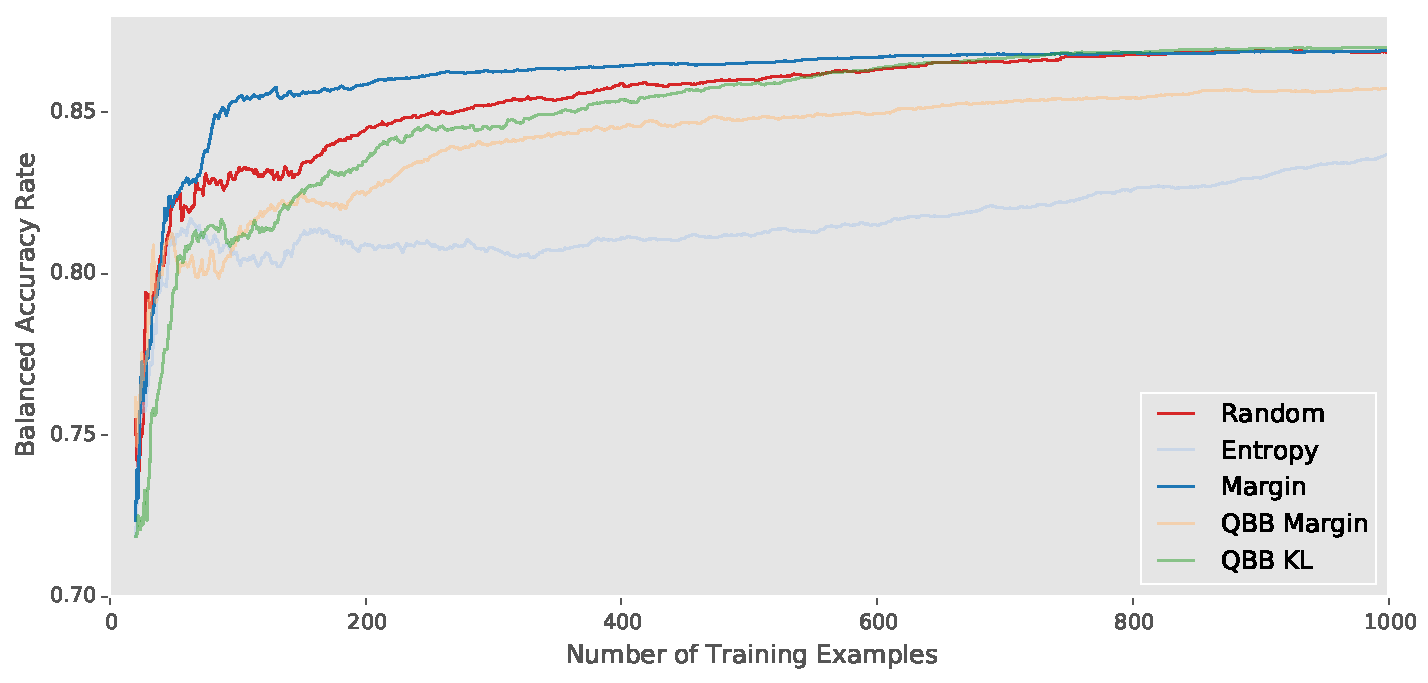
\includegraphics[width=\textwidth]{images/active_logistic_random}
		\caption{Logistic Regression Learning Curve \footnotesize{(Unmodified Unlabelled Pool)}.}
	\end{figure}
\end{frame}



\begin{frame}{Active Learning on the Sloan Dataset}
	\begin{figure}
		\centering
		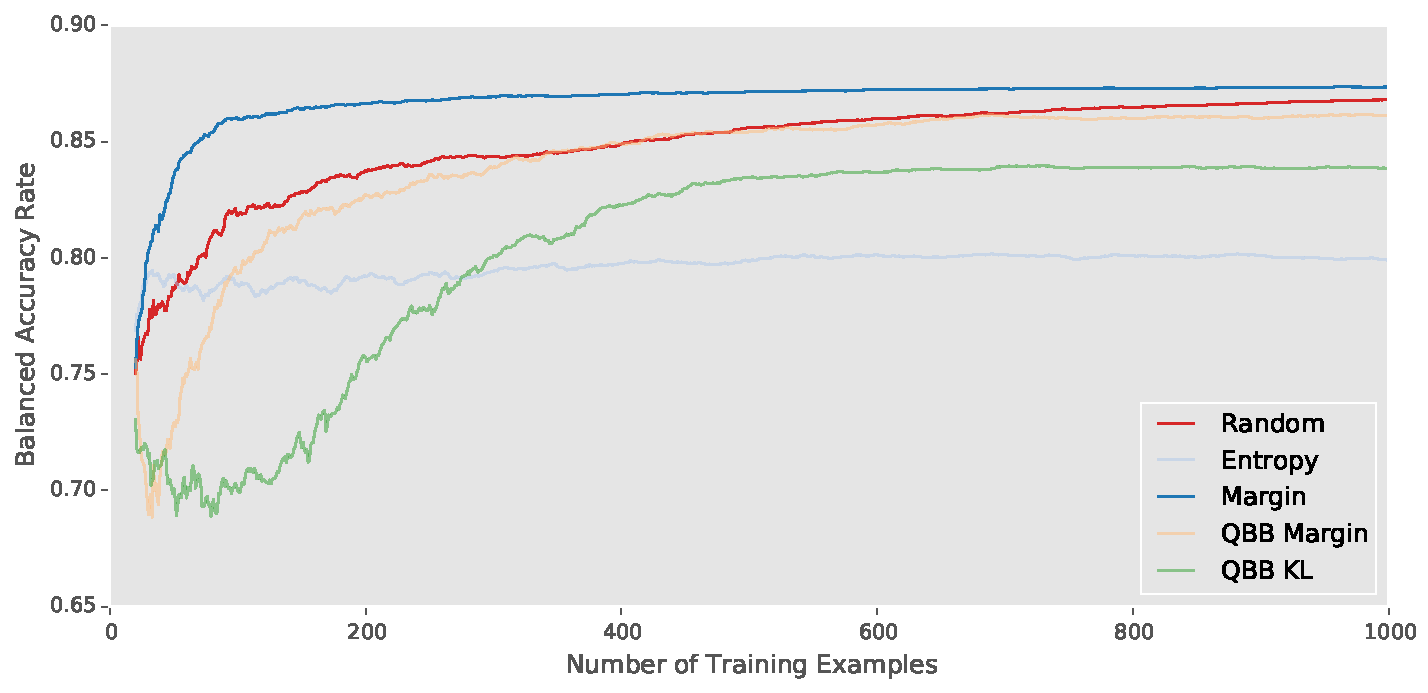
\includegraphics[width=\textwidth]{images/active_logistic_balanced}
		\caption{Logistic Regression Learning Curve \footnotesize{(Balanced Unlabelled Pool)}.}
	\end{figure}
\end{frame}

\begin{frame}{Active Learning with Bandits}
	\begin{itemize}
		\item \textbf{Arms}: clusters of examples in the unlabelled pool.
		\item \textbf{Context}: mean/variance of distance between individual points in the cluster,
		 proportion of labelled points in the cluster, etc.
		\item \textbf{Reward}: cosine distance between the prediction vectors
		of the new and old model.
		\item \textbf{Action}: select cluster at each step to maximise the rewards.
	\end{itemize}
\end{frame}


\begin{frame}{Concluding Remarks}
	\begin{itemize}
		\item Use robust optimisation to take into account of the uncertainty in measurement
		errors.
		\item Theoretical analysis of convergence in multi-class active learning.
		\item My project is hosted at \href{https://github.com/alasdairtran/mclass-sky}{\texttt{github.com/alasdairtran}}.
	\end{itemize}
\end{frame}


\end{document}
